
%(BEGIN_QUESTION)
% Copyright 2010, Tony R. Kuphaldt, released under the Creative Commons Attribution License (v 1.0)
% This means you may do almost anything with this work of mine, so long as you give me proper credit

A pressure transmitter with a remote seal measures the pressure of a gas inside a process vessel.  A pressure gauge directly attached to the vessel registers 19.3 PSI.  The transmitter is located 22 feet 5 inches below this point, with a capillary tube filled with fluid having a specific gravity of 0.94:

$$\includegraphics[width=15.5cm]{i00240x01.eps}$$

How much pressure will the transmitter register?

\underbar{file i00240}
%(END_QUESTION)





%(BEGIN_ANSWER)

The transmitter will measure 28.4 PSI, due to the added pressure of the fluid inside the capillary tube.

%(END_ANSWER)





%(BEGIN_NOTES)

%INDEX% Physics, static fluids: density and specific gravity

%(END_NOTES)


